\documentclass[a4paper,twoside,twocolumn]{article}
\pdfoutput=1

\newif\iftr % \trtrue if for Tech Report
\trtrue     % \trfalse if not for Tech Report
%\newif\ifnony % \nonytrue if nonymised (ie nameful)
%\nonyfalse     % \nonyfalse if anonymised

% Test whether compiler is PDFLaTeX
\usepackage{ifpdf}  % Avoid \newif\ifpdf which clashes with same command
                    % in ifpdf package used by packages like hyperref
\ifpdf
    \usepackage[pdftex]{graphicx}
    \usepackage[colorlinks,linkcolor=blue,citecolor=blue,urlcolor=blue]{hyperref}
    \pdfcompresslevel=9 % Maximum compression
    \DeclareGraphicsExtensions{.pdf}
    % \usepackage[pdftex]{thumbpdf}      % thumbnails for pdflatex
    \pdfadjustspacing=1                % force LaTeX-like character spacing
\else
    \usepackage{graphicx}
    \usepackage[hypertex]{hyperref}  % supports hypertext in PDF but no Acrobat features e.g. bookmarks
\fi
% Common settings for hyperref are made in hyperref.cfg

% Load packages that require graphicx to have been loaded.
\usepackage{todonotes} % clashes with pdftex option below
%\usepackage[disable]{todonotes} % Suppresses todo notes
\newcommand{\bob}[1]{\todo[color=olive!40,inline]{Bob: #1}}
\newcommand{\koen}[1]{\todo[color=red!40,inline]{Koen: #1}}
\newcommand{\asad}[1]{\todo[color=purple!40,inline]{Asad: #1}}
\newcommand{\olivier}[1]{\todo[color=teal!40,inline]{Olivier: #1}}
\newcommand{\vidhi}[1]{\todo[color=orange!40,inline]{Vidhi: #1}}

% Load supported packages
\usepackage{
url       %
,fancyhdr % Fancy Headers
,lastpage % Creates marker with key LastPage, for pxxx of yyy to refer to.
,enumerate % More bullet styles
,amsmath  % AMS maths
,amsfonts % AMS fonts
,amssymb  % AMS symbols
%,moreverb % additional verbatim miscellany
%,amsthm   % AMS theorems defines proof environment
%,calc     % For calculations in length commands
%,newtheorems % Load after hyperref: see below
, enumitem % finer control of lists, e.g. \begin{itemize}[nosep] ... removes spacing
}
%\usepackage[force,almostfull]{textcomp} % Additional symbols, including generic currency
\usepackage[hang]{footmisc} % Hanging indent for footnotes
\setlength\footnotemargin{10pt}
\usepackage{balance}

% Load my personal packages
\usepackage[noindent, arraystretch, fullpage]{setlengths} % [noindent, arraystretch, {fullpage|tightpage|inchrndtext}]{setlengths}
\usepackage{
own         % Defines \newboolean{twocol}
}

% Load my personal packages
%\usepackage{
%newtheorems, % Defines theorem, definition, hypothesis, lemma \& assumption environments
%             % Note: \newtheorem must be used after \usepackage{hyperref} to ensure \theH<counter> is cross-referenced as well as \the<counter>
%}
\usepackage{amsthm}
\newtheorem{assumption}{Assumption}
\newtheorem{requirement}{Requirement}
\newtheorem*{test*}{Test}
\usepackage{xfrac}

\graphicspath{{images/}}

% Preamble metadata---------------------------------------------------
\newcommand*{\metaauthori}{Bob Briscoe}
\newcommand*{\metaauthorii}{Olga Albisser}
\newcommand*{\metashorttitle}{AIMD-Friendliness}
\newcommand*{\metatitle}{Friendliness between AIMD Algorithms}
\newcommand*{\metano}{TR-BB-2021-002}
\newcommand*{\metakeywords}{Data Communication, Networks, Internet, Control, Congestion Control, TCP, Quality of Service, Rate Equality, Steady State, Fairness, Performance, Algorithm, Standards}
\newcommand*{\metahomepage}{\(<\)\href{http://bobbriscoe.net/}{http://bobbriscoe.net/}\(>\)}
\newcommand*{\metamaili}{\href{mailto:research@bobbriscoe.net}{research@bobbriscoe.net}}
\newcommand*{\metamailii}{\href{mailto:olga@albisser.org}{olga@albisser.org}}
\newcommand*{\metaaddress}{}
\newcommand*{\metatel}{Tel. +44 7718 902848}
\newcommand*{\metaversion}{01}
\newcommand*{\metadate}{17 May 2023}

\hypersetup{                       % Set PDF document attributes
     pdfauthor = {\metaauthori and \metaauthorii
     },
     pdftitle = {\metashorttitle},
     pdfsubject = {},
     pdfkeywords = {\metakeywords}
}%

% Set document metadata
\title{\metatitle}%
\author{\metaauthori%
\thanks{\metamaili, %
\metaaddress}%
\ %
\and \metaauthorii%
\thanks{\metamailii}%
}
\date{\metadate}%

% Running headers and footers
\pagestyle{fancy}%
\fancyhf{}%
\fancyhead[LO,RE]{\metashorttitle}%
\fancyhead[LE,RO]{\metano}%
\fancyfoot[LO,RE]{\scriptsize{\copyright~bobbriscoe.net Ltd, 2021-23}}%
%\fancyfoot[LO,RE]{}%
\cfoot{\footnotesize{\scriptsize{Version~\metaversion}}}%
\fancyfoot[RO,LE]{\scriptsize{\thepage~of~\pageref{LastPage}}}%

\fancypagestyle{first}{%
\fancyhead[LO,RE]{}%
\fancyhead[LE,RO]{}%
%\fancyhead[C]{\Large Draft: Limited Review Distribution only}%
\fancyhead[C]{}%
\renewcommand{\headrulewidth}{0pt}%
}%

% Typesetting control
\pretolerance = 150%
%\tolerance = 250%
\tolerance = 5000%
\emergencystretch = 0 em%
% Typesetting overfull/underfull message control
%\hbadness = 150%
\hbadness = 4999%
\hfuzz = 0 pt%

% Set amsmath equation numbering to be relative to containing section
%\numberwithin{equation}{section}
%\newcounter{req}

% Set Sectioning style
%\setcounter{secnumdepth}{3}
%\renewcommand{\baselinestretch}{1.2}
%\renewcommand{\bibname}{References}

% ----------------------------------------------------------------
\begin{document}
\bibliographystyle{alpha}%

% ----------------------------------------------------------------

\maketitle%
\thispagestyle{first}

% ----------------------------------------------------------------
\begin{abstract}
{\small\noindent%
% !TeX root = creno_tr.tex
%=======================================================================================

This paper aims to provide a robust grounding for the additive increase factor used in the `TCP-Friendly' mode of the CUBIC congestion control algorithm.}      % Abstract
\end{abstract}
%\input{ecn-fallback_intr_tr-data}      % Intro
% !TeX root = creno_tr.tex
%=======================================================================================
\section{Introduction}\label{Introduction}

The first IETF RFC to define the CUBIC congestion control algorithm~\cite{Rhee18:Cubic_RFC} was based on the original paper introducing CUBIC~\cite{Ha08:cubic}. For `TCP-friendly' mode, both draw on an equation in an ACIRI technical report~\cite{Floyd00:Eqn_v_AIMD_cc} when they specify the additive increase factor. The derivation of the equation in that technical report assumes a deterministic dropping (or ECN-marking) algorithm at the bottleneck, which limits its applicability. Also the technical report attempts to validate the theoretical formula empirically by simulation using a RED gateway at the bottleneck, but it leads to flow rates that are significantly different (by a factor of more than 2\(\times\)) when they should be the same.

Below, an equation for the additive increase factor is derived without the assumption of deterministic dropping. Instead it is assumed that drops are synchronized between flows, which is typically the case for tail-drop queues. The resulting equation turns out to be the same as that in the technical report~\cite{Floyd00:Eqn_v_AIMD_cc}. However, the derivation here is a straightforward geometric one. It relies on fewer assumptions and no approximations; it considers variation of the RTT explicitly and it does not use loss probability at all.

The present paper is not intended to be ambitious or insightful, just pedestrian and rigorous. \cite{Bansal01:Binom_cc} provides and analyses a wider set of TCP-friendly algorithms, but does not dwell on the simple linear cases analysed here.

\section{Terminology}\label{Terminology}

Nowadays, TCP-friendly mode is more accurately known as Reno-friendly mode, given its flow rate is intended to match that of the Reno congestion control, and given that it is irrelevant which wire protocol is used, whether TCP, QUIC, SCTP, etc. The term C-Reno will be used for Cubic in Reno-friendly mode.

This paper uses the variables defined below:
\begin{description}[nosep]
	\item[\(a\)]: Additive increase factor;
	\item[\(b\)]: Multiplicative decrease factor;
	\item[\(j\)]: Round index;
	\item[\(J\)]: Rounds per sawtooth cycle;
	\item[\(R(j)\)]: Round trip time (RTT);
	\item[\(W(j)\)]: Congestion window;
	\item[\(\check{W}\)]: Minimum \(W\);
	\item[\(r(j)\)]: Packet rate;
	\item[\(X_r\)]: Reno variant of any variable \(X\);
	\item[\(X_c\)]: C-Reno variant of any variable \(X\).
\end{description}

\section{AIMD-Friendliness}\label{AIMD-Friendliness}

Consider two types of Additive Increase Multiplicative Decrease (AIMD) flow with parameters (\(a_r, b_r\)) and (\(a_c, b_c\)) competing at a bottleneck, under the following assumptions:
\begin{itemize}[nosep]
	\item The buffer is large enough not to drain completely, even if all flows reduce simultaneously.
	
	\item All other factors of all the flows, particularly packet size and base RTT, are equal. When flows sharing the same bottleneck queue all have the same base RTT, they all have the same RTT, \(R(j)\),  at every stage, \(j\), of their sawtooth cycles. 	
	
	\item The bandwidth-delay product (BDP) is low enough for all flows to remain in their AIMD mode throughout the cycle.

	\item All the flows have run long enough to converge on a steady state.
\end{itemize}

\begin{figure*}
	\centering
	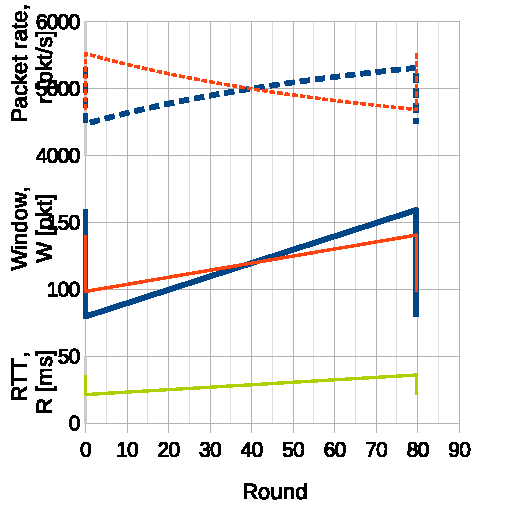
\includegraphics[height=6.5cm]{creno-synch-round}
	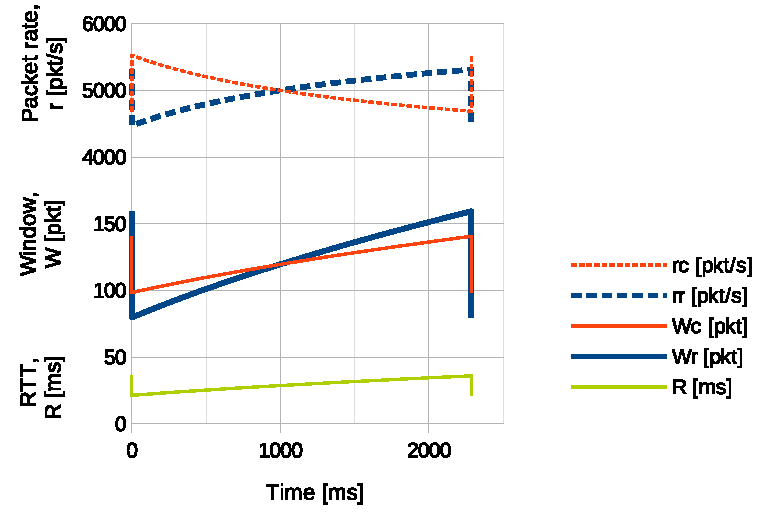
\includegraphics[height=6.5cm]{creno-synch-time}
	\caption{One synchronized sawtooth cycle of C-Reno and Reno plotted wrt.\ round trips (left) and wrt.\ time (right)}\label{fig:creno-synch}
\end{figure*}

% ----------------------------------------------------------------
\subsection{Synchronized (Tail-Drop) Case}\label{Synch}

For this case, it is additionally assumed that:
\begin{itemize}[nosep]
	\item All the flows are synchronized so that, whenever one flow experiences loss the others do too. No assumption is made about how much loss occurs at each congestion event, except that all flows experience it and they only respond to the presence of loss, not its extent.
\end{itemize}

\paragraph{Steady state:} For each flow, the additive increase of a cycle balances with its multiplicative decrease from the max, \(\check{W}/b\), to the min, \(\check{W}\). 
\begin{align}
	a_r J &= \check{W}_r/b_r - \check{W}_r\notag\\
	      &= \check{W}_r(1-b_r)/b_r\label{eqn:ssr}\\
	a_c J &= \check{W}_c(1-b_c)/b_c\label{eqn:ssc}
\end{align}

\paragraph{Flow rate equality:} Given the parameters \(a_r, b_r, b_c\) the aim is to derive \(a_c\) such that each flow's average rate is the same. This is equivalent to each flow transferring the same number of packets over a cycle. 

As a cycle progresses, the RTT grows. So to derive the number of packets transferred over a cycle, the packet rate has to be weighted by the RTT in each cycle before being summed:
\begin{align}
	\sum_{j=0}^{J-1} r_c(j) R(j) &= \sum_{j=0}^{J-1} r_r(j) R(j)\notag\\
	\sum_{j=0}^{J-1} W_c(j) &= \sum_{j=0}^{J-1} W_r(j)\notag\\
	\sum_{j=0}^{J-1} \check{W}_c + a_c j &= \sum_{j=0}^{J-1} \check{W}_r + a_r j\notag\\
	J\check{W}_c +\frac{J^2 a_c}{2} &= J\check{W}_r +\frac{J^2 a_r}{2}\notag\\
\intertext{Dividing through by \(J\) and substituting from \autoref{eqn:ssr} \& \autoref{eqn:ssc}:}
    \check{W}_c \left(1 + \frac{(1-b_c)}{2b_c}\right) &= \check{W}_r \left(1 + \frac{(1-b_r)}{2b_r}\right)\notag\\
	\frac{\check{W}_c}{\check{W}_r} &= \frac{(1+b_r)b_c}{(1+b_c)b_r}\label{eqn:fre}
\end{align}
Returning to the steady state equations, we can divide \autoref{eqn:ssc} by \autoref{eqn:ssr}, then substitute from \autoref{eqn:fre}:
\begin{align}
	\frac{a_c}{a_r} &= 
	                 \frac{\check{W}_c}{\check{W}_r}\frac{(1-b_c)b_r}{(1-b_r)b_c}\notag\\
	                &= \frac{(1-b_c)}{(1+b_c)}\frac{(1+b_r)}{(1-b_r)}\label{eqn:friendly}
\end{align}
Plugging in Reno's AIMD factors, \(a_r=1, b_r=1/2\):
\begin{equation}
                \boxed{a_c = \frac{3(1-b_c)}{(1+b_c)}}\label{eqn:reno-friendly}
\end{equation}
And plugging in the multiplicative decrease factor of C-Reno recommended in \cite{Rhee18:Cubic_RFC}, \(b_c=0.7\):
\begin{align*}
               a_c  &= 9/17\\
                    &\approx 0.53.
\end{align*}

\paragraph{Geometric interpretation:} \autoref{fig:creno-synch} shows one flow each of C-Reno and Reno competing over one synchronized sawtooth cycle. Superficially, the whole derivation of \(a_c\) above can be derived from simple triangle geometry, by drawing congestion window sawteeth that increase linearly wrt.\ round trips (mid-left) then setting the mid-points of the two ramps to the same height. Then \autoref{eqn:fre} gives the ratio between the heights of the bases of the triangles, and \autoref{eqn:friendly} gives the ratio of the heights of the triangles themselves.

\begin{figure*}
	\centering
	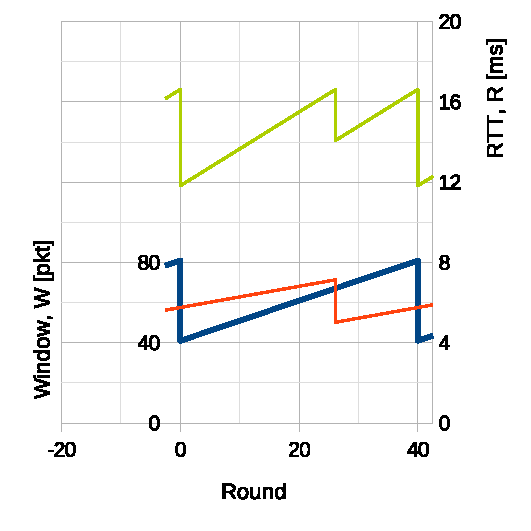
\includegraphics[height=6.4cm]{creno-determ-round}
	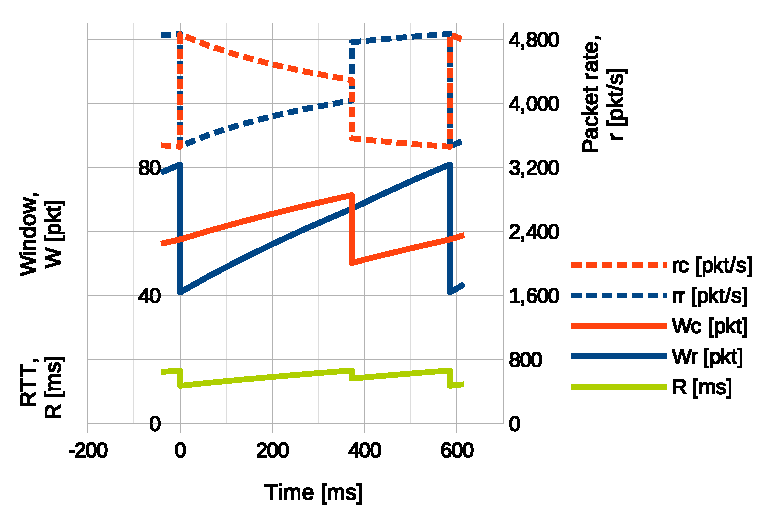
\includegraphics[height=6.4cm]{creno-determ-time}
	\caption{One desynchronized sawtooth cycle of C-Reno and Reno plotted wrt.\ round trips (left) and wrt.\ time (right)}\label{fig:creno-determ}
\end{figure*}

However, it is not enough to merely assert that the average heights of these sawteeth are equal, as \cite{Floyd00:Eqn_v_AIMD_cc} does. It is necessary to start from the goal of equal flow rates averaged over time, as the above analysis does. Given RTT grows throughout the cycle, the plots of flow-rate against time (top right in \autoref{fig:creno-synch}) stretch out more to the right, forming concave curves. It is not at all obvious how to equate the averages of these two curves until they are weighted by round trip duration, which transforms them into the linear plots of window wrt.\ rounds (mid-left).

It is also interesting to note from \autoref{fig:creno-synch} that C-Reno's packet rate \emph{decreases} as its window increases over the sawtooth. This is because the competing Reno flow causes the RTT to grow faster than would be the case with only C-Reno flows. If the buffer is not deep enough to hold all the synchronized sawteeth, it will be empty during the early part of the sawteeth. Then C-Reno will miss its highest packet rate and Reno will miss its lowest, so C-Reno's average packet rate will be lower than Reno's. 

This might help explain the simulation results with a tail-drop queue in Floyd's report~\cite{Floyd00:Eqn_v_AIMD_cc}, where C-Reno's packet rate was lower than the theory predicted.

% ----------------------------------------------------------------
\subsection{Desynchronized (AQM) Case}\label{AQM}

For this case, instead of the assumption of synchronization, it is assumed that:
\begin{itemize}[nosep]
	\item As the queue grows, Active Queue Management (AQM) at the bottleneck selects single packets to drop or mark, so that the congestion responses of each flow tend not to coincide.\footnote{In desynchronized cases, the RTT varies much less than in synchronized cases---on average the amplitude is respectively \(1/\sqrt{n}\) vs.\ \(n\) times that of a single flow, where \(n\) is the number of flows~\cite{Appenzeller04:Sizing_buffers}. Therefore, the first assumption (that the buffer is large enough not to drain completely) is much more likely to hold in desynchronized cases.}
\end{itemize}

The AQM case is harder to analyse than the synchronized case with tail-drop. Superficially, one could use the transformation from equal average flow rates (wrt.\ time) into equal window (wrt.\ rounds). However, there is no guarantee that the number of rounds per cycle, \(J\) is the same in each case.

If we assumed it was, we would end up with \autoref{eqn:reno-friendly} for C-Reno's additive increase factor \(a_c\). Then, as shown in \autoref{fig:creno-determ}, the phasing between the sawteeth would evolve so that the queue reached roughly the same depth before each reduction, i.e.\ the tips of the RTT sawteeth will all align at roughly the same level---the operating point of the AQM. 

However, although \autoref{fig:creno-determ} shows the sawtooth reductions alternating Reno -- C-Reno -- Reno, this need not be the case. At 400\,ms in the top-right plot, the ratio between C-Reno's and Reno's packet rates is about 51:49. So it is nearly as likely that the AQM will hit a Reno packet as a C-Reno packet, causing Reno to reduce twice in a row. If the AQM did hit C-Reno around 400\,ms, at around 600\,ms the ratio would be about 42:58, making Reno more likely to be hit. Overall, if \(a_c\) is set for the synchronized case, an AQM is likely to hit Reno somewhat more often than C-Reno.

This runs counter to the simulation results using the RED AQM in Floyd's report~\cite{Floyd00:Eqn_v_AIMD_cc} where the throughput of C-Reno was 70\% of that of competing Reno flows when C-Reno used \(b_c=7/8\) and \(a_c\) was set according to  \autoref{eqn:reno-friendly}.
      % Body
%\input{creno_eval_tr-data}      % Evaluation
%\input{creno_relwk_tr-data}     % Related work
% !TeX root = creno_tr.tex
%=======================================================================================
%\section*{Acknowledgements}\label{Acks}
%The experiments in \autoref{fig:creno-v-reno-PIE} were conducted and plotted by Olga Albisser.

%=======================================================================================
\section{Conclusion}\label{Conclusion}

This report provides:
\begin{itemize}[nosep]
	\item a formula (\autoref{eqn:reno-friendly}) for the additive increase parameter of an AIMD algorithm as a function of its chosen multiplicative decrease factor that should maintain an equal flow rate with another AIMD flow, specifically a Reno flow. 
	
	\item a derivation of the formula that relies on fewer assumptions and is more rigorous than that in Floyd \emph{et al}~\cite{Floyd00:Eqn_v_AIMD_cc}. It applies to tail drop buffers whereas that in Floyd \emph{et al} relied on an AQM with deterministic marking. Nonetheless the formula turns out to be the same.
	
	\item a testbed validation of the formula (at least for the case where the MD factor is 0.7) over a range of 25 different path characteristics (5 rates and 5 base RTTs) with a tail-drop bottleneck buffer.
	
	\item a testbed evaluation of the formula over the same range of scenarios but with a PIE AQM at the bottleneck. This shows that the AI factor works correctly over a PIE AQM, even though it was derived assuming tail-drop.
\end{itemize}

These result show that, with the widely deployed decrease factor of \(b_c=0.7\), the Reno-Friendly mode in CUBIC is sufficiently well modelled by \autoref{eqn:reno-friendly} that the Additive Increase factor it produces (\(a_c = 0.53\)) ensures that TCP CUBIC competes roughly equally with Reno across its intended operating range, whether with a tail-drop queue or a single-queue AQM (PIE) at the bottleneck.      % Tail pieces (discussion, conclusions, plans, acks)
% ----------------------------------------------------------------

%\onecolumn%
%\clearpage
\newpage
\addcontentsline{toc}{section}{References}

%\newpage
{%
%\footnotesize%
\scriptsize%
\bibliography{creno}}

% ----------------------------------------------------------------
%\clearpage
%\twocolumn%
%\appendix
%\input{creno_appx_tr-data}      % Appendix
%\onecolumn%
% ----------------------------------------------------------------

\onecolumn%
\addcontentsline{toc}{part}{Document history}
\section*{Document history}

\begin{tabular}{|c|c|c|p{3.5in}|}
 \hline
Version &Date &Author &Details of change \\
 \hline\hline
00A          &29 Sep 2021&Bob Briscoe &First draft.\\\hline%
00B          &01 Oct 2021  &Bob Briscoe &Added geometric interpretation and deterministic case.\\\hline%
00C          &03 Aug 2022  &Bob Briscoe &Added shallow buffer case, empirical results over PIE and discussion of the applicability of the synchronized loss model. Added Acks section. Altered analysis to use max window not min.\\\hline%
00D          &08 Aug 2022  &Bob Briscoe &Added explicit step at \autoref{eqn:p_ratio1} that was previously implicit.\\\hline%
00E          &16 Mar 2023  &Bob Briscoe &Added text around results in \S\,\ref{empirical-pfifo}. Improvements throughout. Expanded conclusions.\\\hline%
\metaversion &\metadate  &Bob Briscoe &Issued without further changes.\\\hline%
\hline%
\end{tabular}

\end{document}

% ----------------------------------------------------------------

%Useful section headers
%% ================================================================
%\section{}\label{creno_}
%
%% ----------------------------------------------------------------
%\subsection{}\label{creno_}
%
%% - - - - - - - - - - - - - - - - - - - - - - - - - - - - - - - -
%\subsubsection{}\label{creno_}
